\documentclass{article}

\usepackage{graphicx}
\usepackage{booktabs}
\usepackage{gensymb}
\usepackage[section]{placeins}
\usepackage[parfill]{parskip}

\setcounter{secnumdepth}{0}

\begin{document}

\begin{figure}[h!]
 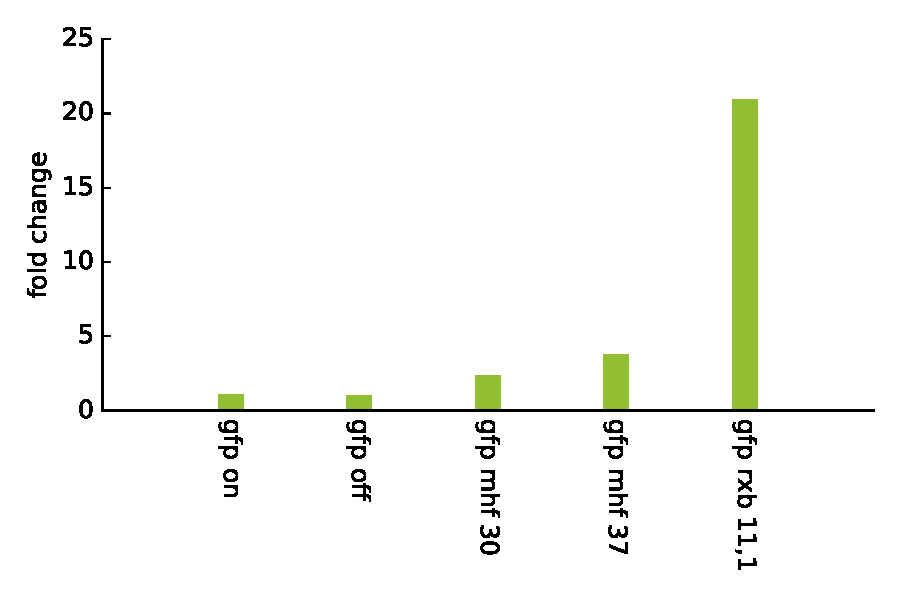
\includegraphics[width=\textwidth]{in_vitro_fold_change.pdf}
 \caption{Results from the \emph{in vitro} Cas9 cleavage experiment with our 
 inducible sgRNAs in the context of four different spacers.  The ``on'' and 
 ``off'' constructs are the positive and negative controls, respectively.  The 
 negative control has two mutations in the nexus domain that render it 
 non-functional.  The dark blue bars represent the ``gfp'' spacer we use in our 
 bacterial CRISPRi assay.  All three of our designs work well with this spacer 
 in that assay.  The light blue bars represent the three spacers you gave us to 
 test.  Each is labeled by its first three nucleotides.  ``CCG'' is the spacer 
 that's already been tested in mammalian cells; ``CAG'' and ``CCT'' are the two 
 that haven't.  The grey axis on the right corresponds to the arrows.  The tail 
 of each arrow shows what percent of the DNA was cleaved without theophylline, 
 and the head shows what percent was cleaved with.}
\end{figure}

\begin{figure}[h!]
 \includegraphics[width=\textwidth]{20170124_cleave_cf_spacers_with_controls_1.png}
 \includegraphics[width=\textwidth]{20170124_cleave_cf_spacers_with_controls_2.png}
 \caption{Raw data from the \emph{in vitro} Cas9 cleavage experiment.  Each 
 reaction contained 30\,nM Cas9, 150\,nM \emph{in vitro} transcribed sgRNA, 
 3\,nM target DNA, and either water (in the lanes labeled ``-'') or 10\,mM 
 theophylline (in the lanes labeled ``+'').  The reactions were incubated at 
 37\degree{}C for 1\,h, then quenched by the addition of RNase~A and 
 proteinase~K.  The target DNA is 4\,kb and the cleavage site is  roughly in 
 the middle, so the 4\,kb and 2\,kb bands are the uncleaved and cleaved DNA 
 respectively.}
\end{figure}

\begin{table}[h!]
 \centering
 \begin{tabular}{ll}
  \toprule
  Name    & Sequence             \\
  \midrule
  gfp     & \texttt{CATCTAATTCAACAAGAATT} \\
  ``CCG'' & \texttt{CCGGCAAGCTGCCCGTGCCC} \\
  ``CAG'' & \texttt{CAGGGTCAGCTTGCCGTAGG} \\
  ``CCT'' & \texttt{CCTCGAACTTCACCTCGGCG} \\
  \bottomrule
 \end{tabular}
 \caption{The spacer sequences tested in this experiment.}
\end{table}

\section{Discussion}

All three of the designs tested here (``rxb 11,1'', ``mhf 30'', and ``mhf 37'') 
work equally well in our bacterial CRISPRi assay, but ``mhf 30'' seems to work 
distinctly worse than the others in this cleavage assay.  We're not sure why 
this is.

We detected no cleavage for any of the designs with the ``CCG'' spacer, with or 
without theophylline.  We used \texttt{RNAfold}, an RNA secondary structure 
prediction program, to look for base-pairing between the ``CCG'' spacer and the 
sgRNA that could explain the lack of activity, but no such base-pairing was 
predicted.  The positive control for this spacer also has relatively weak 
cleavage, so it may be that this spacer just doesn't work that well in our 
assay and that we didn't detect any cleavage because the dynamic range is too 
small.  

In contrast, we observed reasonable activity for the ``rxb 11,1'' and ``mhf 
37'' designs with the ``CAG'' and ``CCT'' spacers.  We believe that this 
activity is promising enough to justify testing these designs with these 
spacers in the mammalian cell assay.  Even for these guides, however, it's 
worth noting that the positive controls only achieved about 50\% cleavage.

The conditions we used in this assay probably don't correlate at all to the 
conditions in the mammalian cell assay.  We had a 10-fold excess of Cas9 over 
target DNA, an 5-fold excess of sgRNA over Cas9, and a 66-fold excess of 
theophylline over sgRNA.  In other words, we expect that every interaction in 
our system was saturated.

\end{document}
